\documentclass[conference]{IEEEtran}
\usepackage{listings}
\usepackage{float}
\usepackage{graphicx}
\usepackage{xcolor}
\usepackage{cite}
\usepackage{capt-of}

\title{Nanowire Interconnects}
\author{Nicholas Sica}
\date{November 9, 2020}
\begin{document}
\maketitle

\begin{abstract}
As devices continue to decrease in size, new technologies are being explored as alternatives to the traditional interconnects.
Among these are nanowire, optical, and graphene interconnects are the three biggest contenders as a replacement.
In this survey paper, nanowire interconnects and their relation to the other options will be explored as well as other uses
that can be exploited from them.
\end{abstract}
\enlargethispage{-10cm}
\noindent\begin{picture}(0,0)
    \put(0,-370){\begin{minipage}{\textwidth}
    \centering
        \rule{\textwidth}{0cm}
        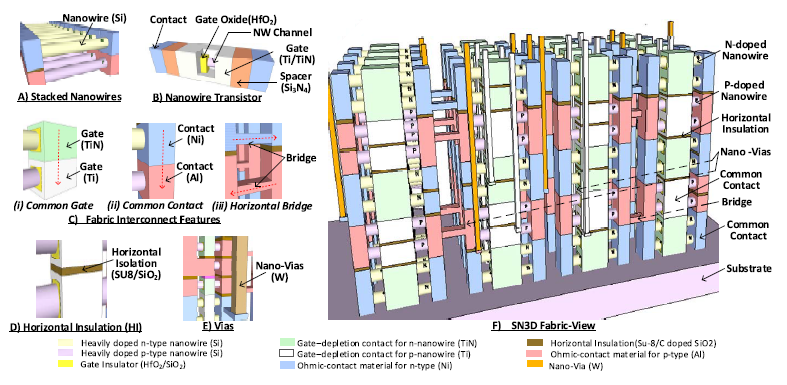
\includegraphics[width=\textwidth]{figures/3d_cmos.PNG}
        \captionof{figure}{SN3D fabric core components. (A) stacked nanowires. (B) Junction-less transistor surrounded by gate. (C) Different Interconnects
        (D) Horizontal isolation. (E) Vias. (F) Fabric of all components \cite{8387522}.}\label{fig:3d_cmos}
    \end{minipage}}
\end{picture}
\section{Introduction}
While scaling down CMOS designs, researchers are looking for the best material to use for the interconnects of the device.
Every material brings different, interesting properties to the table and many researchers are looking for alternatives to the
traditional copper interconnect \cite{7968937}, while others are seeing what they can do with copper or really most nanowire
materials. Nanowire interconnects provide significant improvements in power and performance when using them for 3-D CMOS
design as opposed to the traditional approach \cite{8387522}. They also allow for new technologies to be released, like
integrated circuits that can self-repair \cite{8423678}, or even building logic right into the interconnects \cite{5510748}. The first
section will discuss the biggest alternative to copper, ruthenium, and how it compares to copper when used as a nanowire
interconnect. The section will also discuss methods in which placing metal interconnects will not be as wasteful, thus
using less of the more expensive metals. The next section will discuss
advancements in 3-D CMOS fabrication due to nanowire interconnects and a whole method that was designed with nanowire
interconnects. The second to last section will talk about configurable interconnects and replacing vias with transistors
made out of nanowires. Lastly, research into self-repairing circuits made from nanowire interconnects, memristors, and
permanent components which allows a designer to fix faulty sections of a circuit will be looked at.

\enlargethispage{-10cm}
\section{Nanowire 3-D CMOS Fabrication}
The use of nanowires causes 3-D CMOS design to improve dramatically, but causes a lot of what is expected to change in the process.
The 3-D CMOS approach researched is called stacked horizontal nanowire-based 3-D CMOS approach, or SN3D. This 3-D CMOS approach
allows for higher density packing, fine-grained routing, reduced interconnect lengths, and better control of transistors in which
the gate is surrounding them \cite{8387522}. Fig.~\ref{fig:3d_cmos} shows the basic structure of different parts of the CMOS fabric.
The idea of using a nanowire as a transistor, which is done in this method, is discussed in greater detail in the next section.
A bunch of different designs were created and the new 3-D CMOS method was found to have a way smaller area, less power consumption,
and a shorter delay when it came to a two input NAND, a full adder, and a four bit adder. It also maintained this lead even when 
the sizing of the transistors changed, only being beat in area at the 45nm node. 
The fabrication of these designs is radically different because a lot of the nanowire needs to be placed on air, which is an issue
due to nothing holding the nanowire up.

\section{Ruthenium Nanowire Interconnects}
The big contenders in alternative metals when it comes to replacing copper are platinum-group metals or more specifically,
ruthenium \cite{7968937}. The biggest advantage of ruthenium over copper is the current carrying capability of the metal \cite{7968937}.
As shown in Fig.~\ref{fig:curr_ruth}, ruthenium has a current carrying capability between 530 and 720MA/cm\textsuperscript{2}. 
\begin{figure}[!htb]
    \centering
    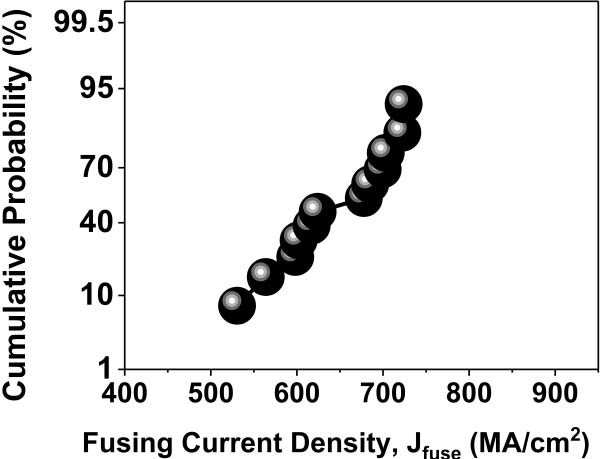
\includegraphics[width=\linewidth]{figures/curr_ruth.png}
    \caption{Fusing current density of Ru nanowires \cite{7968937}.}\label{fig:curr_ruth}
\end{figure}
This beats copper's carrying capacity of 100MA/cm\textsuperscript{2} greatly and shows the biggest gain when it comes to ruthenium
\cite{7968937}.
Ruthenium also did not break down when the temperature changed which proved it could be used in very hot environments without any issue
when it comes to the circuit functioning correctly.
The biggest trade-off of a metal like ruthenium is its cost. It is due to the cost of ruthenium and other metals similar to it that
methods of saving material while placing them are being researched heavily. The most promising method is gas-phased electrodeposition and
the general method involves using an inert gas to transfer nanoparticles from a spark to where the metal is intending to go. The general
steps of placing a nanowire using gas-phased electrodeposition is shown in Fig.~\ref{fig:electrodepo} while the old method is shown in
Fig.~\ref{fig:inter_fab}.
\begin{figure}[!htb]
    \centering
    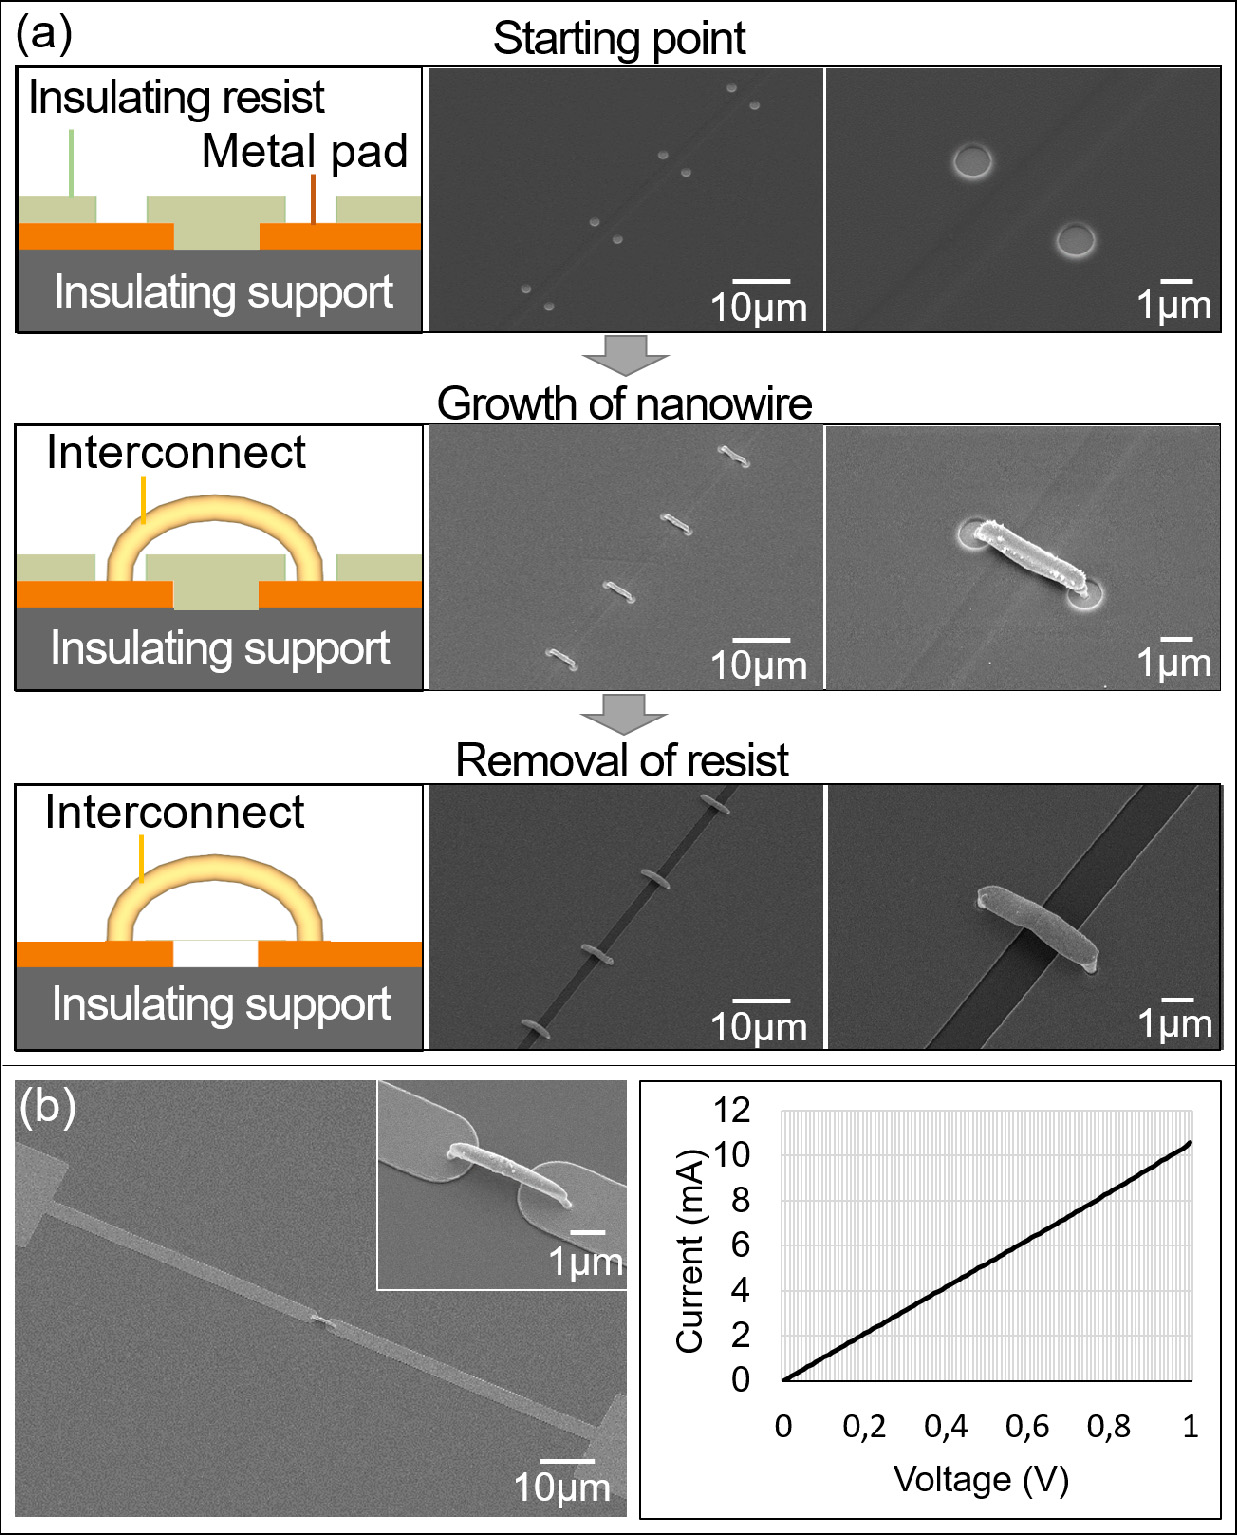
\includegraphics[width=\linewidth]{figures/electrodepo.png}
    \caption{(a) shows the phases in electrodeposition of nanowire materials (b) shows the current-voltage characteristic of a single bridge
    \cite{8605857}.}\label{fig:electrodepo}
\end{figure}
\begin{figure}[!htb]
    \centering
    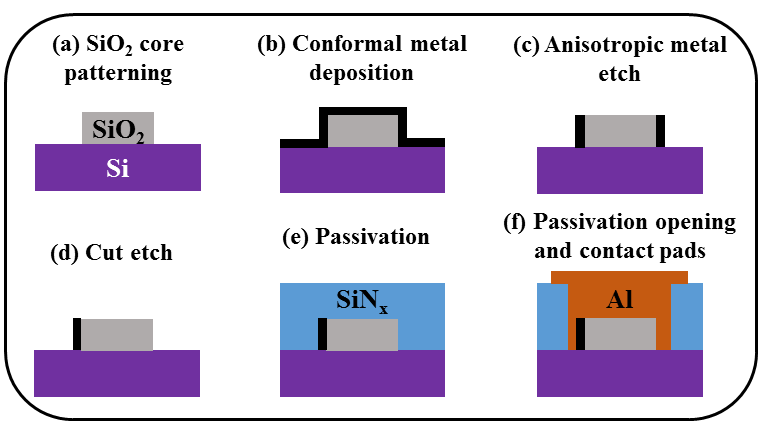
\includegraphics[width=\linewidth]{figures/inter_fab.png}
    \caption{Flow to fabricate nanowires \cite{7968937}.}\label{fig:inter_fab}
\end{figure}
The old method had a yield of about 53\% \cite{7968937} while the new method has a yield of about 95\% \cite{8605857}
when it came to the amount of metal used. The new method of placing nanowires also allows for the self alignment of pads, which allows for
the pads to not have to be perfectly lined up to create a connection between the two. This method also allows for two arbitrary points of a
design to be connected without any modification to the layout which could lead to further design improvements.

\section{Reconfigurable Interconnects}
Vias in a 3-D CMOS design are used to connect different layers of the design together and
even allow for 3-D CMOS designs to be realized in a more condensed form. Fig.~\ref{fig:nanowire_transistor}
shows a nanowire transistor inserted where a via would be. The general method of creating these
reconfigurable interconnects is to grow silicon and put a metal on the tips. Gold would be best,
but is generally avoided by semiconductor manufacturers which leads to research into alternatives,
most notably copper \cite{5510748}. The use of these silicon nanowire interconnects can possibly
allow designers to disable areas of their device by using it like a transistor. Nanowire transistors
are even used in the 3-D CMOS fabrication research discussed in the previous section.
\begin{figure}[!htb]
    \centering
    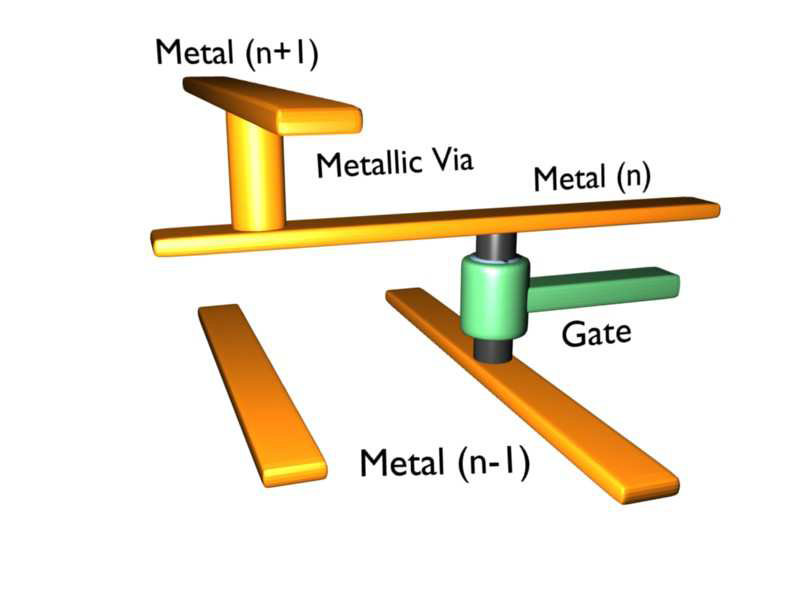
\includegraphics[width=\linewidth]{figures/nanowire_transistor.png}
    \caption{Nanowire transistor in interconnect \cite{5510748}.}\label{fig:nanowire_transistor}
\end{figure}

\section{Self-Repairing Interconnects}
The idea behind self-repairing interconnects builds off a field programmable nanowire interconnect (FPNI)
which is basically an field programmable gate array (FPGA) built using nanowires. Fig.~\ref{fig:fpni}
shows the basic layout of an FPNI device. Self-repair usually occurs in several steps. The first step
being the device identifies faulty areas, next isolates them by putting switching elements in, and finally
replaces them with a working unit. The device has a permanent layer and an FPNI layer connected
using memristors. As the device identifies areas that need to be replaced, the FPNI layer reconfigures itself
to use different paths between the permanent parts of the design which allows for the faulty areas to be
avoided \cite{8423678}. This could also lead to allowing a designer to switch out the faulty areas for new,
working parts. The mixture of FPGAs and ASICs (application-specific integrated circuit) allow for a much
more versatile technology, one that allows for great reconfigurability of certain areas. The device gets
the speed and performance of an ASIC while maintaining the ability to
use different pathways in case of a fault in the current one.
\begin{figure}[!htb]
    \centering
    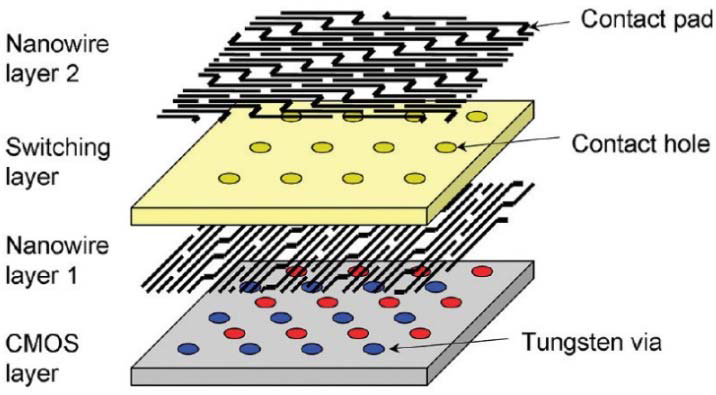
\includegraphics[width=\linewidth]{figures/fpni.png}
    \caption{Breakdown of eacch layer of FPNI technology \cite{8423678}.}\label{fig:fpni}
\end{figure}

\section{Conclusion}
There is much discussion and research when it comes to nanowire interconnects as
the best material needs to be chosen going forward as an industry standard. This
issue will only get more prominent as the devices grow smaller and smaller due
to the limits of materials already being used as interconnects. The discovery of
different properties that different materials possess as well as new technologies
the materials enable will likely lead to certain industries leaning towards using
a certain material over others. The impact of the interconnect is a huge one and it is important
that the trade-offs of every material is closely examined as to make the right choice.
The improvements discussed by a 3-D CMOS fabrication process using nanowire interconnects
is also promising and could allow for faster and more compact designs. Given the adoption
of new materials and methods to not use so much of the expensive materials, integrated
circuits could get a lot faster and smaller, given that nanowire interconnects are adopted.
\bibliographystyle{IEEEtran}
\bibliography{ref}

\end{document}
%%% Local Variables:
%%% mode: latex
%%% TeX-master: t
%%% End:
